\documentclass[tikz, border=1cm]{standalone}
\begin{document}
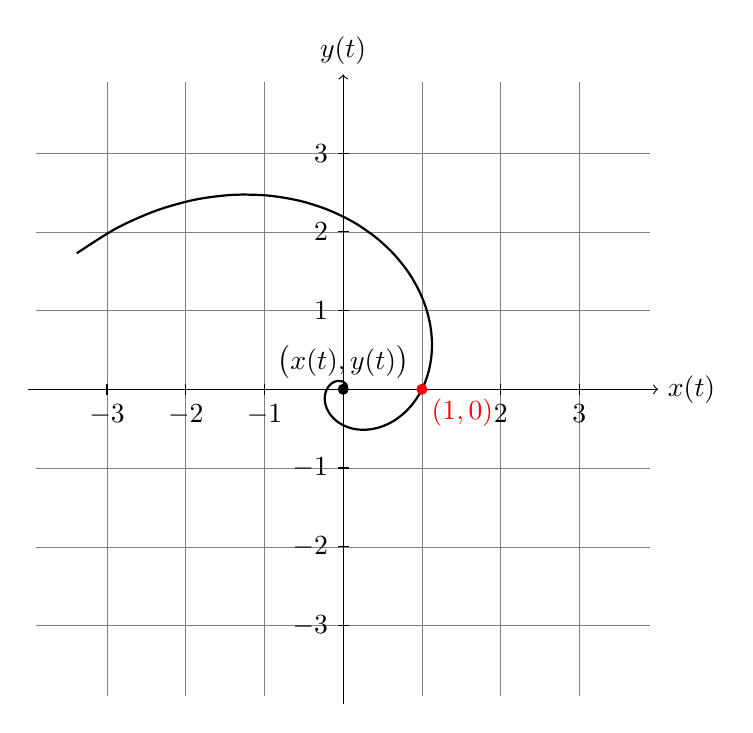
\begin{tikzpicture}
\draw[gray, very thin] (-3.9,-3.9) grid (3.9,3.9);
\draw[->] (-4,0) -- (4,0) node[right] {$x(t)$};
\draw[->] (0,-4) -- (0,4) node[above] {$y(t)$};
\foreach \pos in {-3,-2,-1,2,3}
\draw[shift={(\pos,0)}] (0pt,2pt) -- (0pt,-2pt) node[below] {$\pos$};
\foreach \pos in {-3,-2,-1,1,2,3}
\draw[shift={(0,\pos)}] (2pt,0pt) -- (-2pt,0pt) node[left] {$\pos$};
\fill (0,0) circle[radius=2pt];
\draw[thick, variable=\t, domain=-0.2:7, samples=100, trig format=rad, smooth]
plot ( {e^(-\t)*(-2*cos(2*\t)+2.3817218*sin(2*\t))} , {e^(-\t)*(2.3817218*cos(2*\t)+2*sin(2*\t))} )
node[above] {$\bigl(x(t),y(t)\bigr)$};
\fill[red] (1,0) circle[radius=2pt] node[below right] {$(1,0)$};
\end{tikzpicture}
\end{document}